\chapter{Deep Learning for CSI Estimation}
\label{chap:sph_norm}

In this chapter, we will discuss important aspects of successfully applying deep learning to MIMO CSI estimation. In Section~\ref{sect:dl_overview}, we provide a basic overview of deep learning concepts that are pertinent to the task of CSI estimation. In Section~\ref{sec:data-preprocessing}, we discuss data pre-processing techniques and the applications of domain knowledge that have enabled successful application of. In Section~\ref{sect:sph_norm}, we describe our proposed CSI pre-processing technique, spherical normalization, which boosts estimation accuracy without changing computational complexity. 

\section{Deep Learning Background}
\label{sect:dl_overview}

This section provides a brief overview of relevant deep learning concepts employed in this work, including convolutional neural networks (CNNs), autoencoders, and unsupervised learning.

\textbf{Deep learning (DL)} is a subset of machine learning (ML), a broad class of algorithms which use data to ``fit'' models for prediction or classification tasks. The three predominant learning frameworks are supervised learning, unsupervised learning, and reinforcement learning. In the works proposed, we focus on \emph{unsupervised learning}, which seeks to find a compressed representation of the data without labels (see Chapter 14 of \cite{ref:Hastie2016Elements} for an overview).

\textbf{Convolutional Neural Networks}: A neural network is a machine learning algorithm with multiple \emph{layers} of parameterized linear functions followed nonlinear functions (typically referred to as `activation' functions). The parameters for these layers can be updated via a stochastic optimizer (e.g., \cite{ref:Kingma2014ADAM}), and given enough layers, such networks can achieve arbitrarily accurate functional approximation \cite{ref:Hecht1992TheoryBackprop}. In recent years, neural networks with convolutional layers have established state-of-the-art performance in computer vision tasks such as image classification \cite{ref:Sabour2017Dynamic} and segmentation \cite{ref:He2017Mask}.

\begin{figure}[!hbtp]
\centering
\def\svgwidth{0.8\columnwidth}
\input{images/autoencoder_schematic.pdf_tex}
\caption{Abstract schematic for an autoencoder operating on CSI matrices $\mathbf H$. The encoder learns a latent representation, $\mathbf Z$, while the decoder learns to reconstruct estimates $\hat{\mathbf H}$.}
\label{fig:autoencoder_schematic}
\end{figure}

A common architecture for deep unsupervised learning is the \emph{autoencoder} (see Fig.~\ref{fig:autoencoder_schematic} for a generic example). Trained end-to-end on input data, an autoencoder is comprised of an encoder and a decoder which jointly learn a compressed latent representation ($\mathbf Z$) and an estimate of the input ($\hat{\mathbf H}$). By choosing $\mathbf Z$ to have lower dimension than the input, the network is forced to learn a ``useful'' summary of the input data. The typical objective function for such a network is the mean squared error (MSE),
\begin{align*}
\underset{\theta_e, \theta_d}{\text{argmin}}\; \frac 1N \sum_{i=1}^N\Arrowvert \mathbf H_i - g(f(\mathbf H_i, \theta_e), \theta_d) \Arrowvert^2.
\end{align*}
We optimize network parameters $\vec \theta_e, \vec \theta_d$ by backpropagation and a stochastic optimization algorithm (e.g., stochastic gradient descent, ADAM).

\textbf{Computational Complexity}: Given the number of layers and operations involved in any deep learning algorithm, measuring the \textbf{computational complexity} of these algorithms is important. Two metrics that are commonly used in deep learning literature are:

\begin{enumerate}
	\item \textbf{Floating point operations (FLOPs)}: FLOPs provide a measure of the compute consumed by a given layer or mathematical operation in a network. A single FLOP is defined as any arithmetic operation between floating point numbers (e.g., addition, multiplication) or any assignment of a floating point value.
	\item \textbf{Parameters}: The number of parameters in a deep learning network determines the storage cost for inference\footnote{The size of the dataset will contribute towards the storage cost but only during training/evaluation.}. The number of parameters in a typical deep learning model can be anywhere from millions (e.g., ResNet architectures \cite{ref:he2016identity}) to billions (e.g., GPT-3 \cite{ref:brown2020language}).
\end{enumerate}

See Appendix~\ref{appdx:complexity} for a more exhaustive discussion of common layers/operations used in deep networks and their corresponding computational complexity.

% For data with multiple input features of different scales. In ML curricula, this is often illustrated using the iris dataset \cite{ref:anderson1936species,ref:fisher1936use}), which contains .

\section{Data Pre-processing for CSI Data} \label{sec:data-preprocessing}

The success of machine learning tasks relies on proper \emph{data pre-processing}, a sequence of transformations used on the input data before fitting a model. In any machine learning task, data pre-processing is necessary to ensure that the scales of input features are similar. In deep learning, three important pre-processing techniques are domain transformations, truncation, or normalization, and here we will explore the choices in pre-processing that different authors have made based on domain knowledge of MIMO CSI data.

\subsection{Sparse Basis for CSI} \label{sect:sparse-csi}

\begin{figure}[htb]
	\centering
	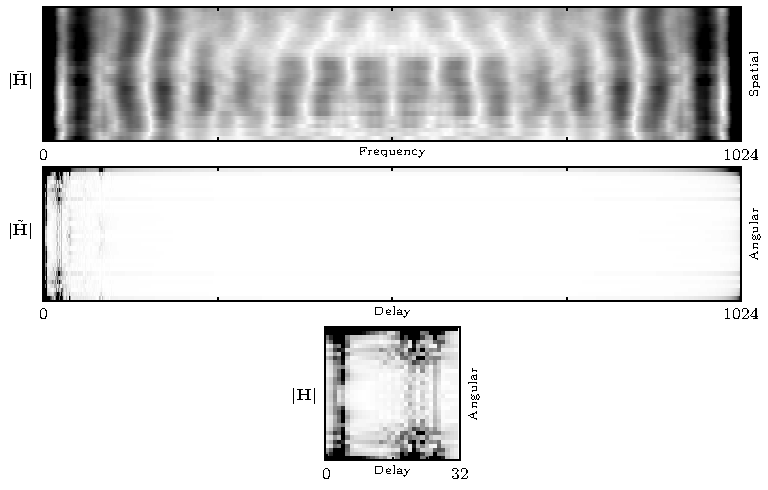
\includegraphics[width=.8\textwidth]{batch17_sample0_freqvsdel_truncatevsfull.pdf}
	\medskip
	\caption{Magnitude of spatial-frequency ($\bar{\mathbf H}$), angular-delay ($\tilde{\mathbf H}$), and truncated angular-delay ($\mathbf H$) representations for a single random channel from the outdoor COST2100 dataset.}
	\label{fig:freq-vs-delay}
\end{figure}

The first type of data pre-processing we consider is a domain transformation, the discrete Fourier transform in particular. While the \textbf{spatial-frequency} representation $\bar{\mathbf H}$ is used for beamforming at the transmitter, the number of non-zero elements is comparatively large. Given the dimension of $\bar{\mathbf H}$, feeding back entire CSI matrices is impractical. Instead, we seek a compressed representation of a sparse transformation. The sparse representation we consider is the angular-delay representation of CSI matrices \cite{ref:sayeed2002deconstructing}. Denote the unitary inverse DFT for the spatial (frequency) axis as $\mathbf F_a \in \mathbb C^{N_b \times N_b}$ ($\mathbf F_d^H \in \mathbb C^{N_f \times N_f}$), and denote the spatial-frequency CSI matrix as $\bar{\mathbf H}$. The angular-delay domain representation $\tilde{\mathbf H}$ is given as % $\mathbf F \in \mathbb C^{(n_f \times n_f)}$ ($\mathbf F^H \in \mathbb C^{(n_f \times n_f)}$)
\begin{align*}
	\tilde{\mathbf H} &= \mathbf F_d^H \bar{\mathbf H} \mathbf F_a.
\end{align*}
The delay spread of the resulting $\tilde{\mathbf H}$ can typically be captured with a small number of delay elements (see Figure~\ref{fig:outdoor_energy_cdf}), so we restrict our attention to the first $R_d$ elements of $\tilde{\mathbf H}$, resulting in a truncated angular-delay matrix which we denote as $\mathbf H \in \mathbb C^{(R_d\times N_b)}$ for the downlink channel state. An illustrative example of this truncation can be seen at the bottom of Figure~\ref{fig:freq-vs-delay}. % (uplink) ($\mathbf H_u \in \mathbb C^{(R_d\times N_b)}$) 

\begin{figure}[!hbtp]
    \centering
    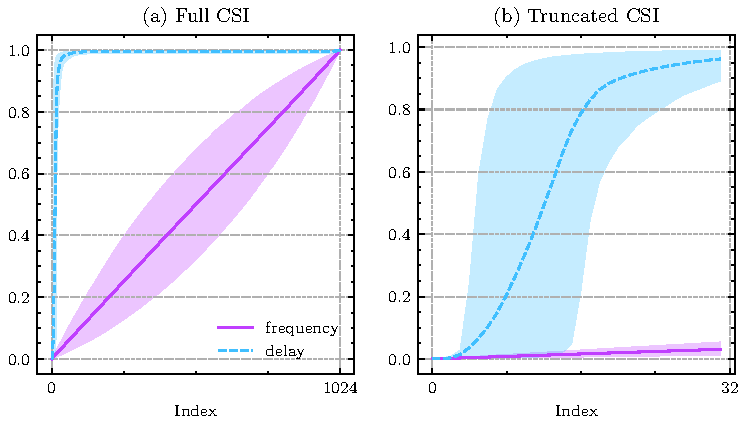
\includegraphics{trunc_energy_cdf_horiz.pdf}
    \caption{Energy CDF for 5000 
    CSI samples
of 32 antennas and 1024 subcarriers, generated
  from 
COST2100 outdoor models described in Section \ref{sect:channel_model}.
Mean percentage of energy in CSI matrix up to index is shown with 90\% confidence intervals. The index denotes the amount of energy accounted for up to the corresponding frequency/delay element. The truncated angular-delay CSI contains a mean energy of 96.2\% (c.i. 89.2\%, 99.1\%), while the truncated frequency-spatial CSI only contains a mean energy of 3.1\% (c.i. 1.2\%, 5.4\%).} 
    \label{fig:outdoor_energy_cdf}
\end{figure}

% Rather than learning a lower dimensional representation of $\bar{\mathbf H}$, the authors of \cite{ref:csinet} chose to compress the \textbf{angular-delay} domain representation of CSI, $\tilde{\mathbf H}$. Given the sparsity of the angular-delay matrices, many works using this basis choose to compress and feedback a truncated version of the CSI matrices, $\mathbf H \in \mathbb R^{R_d \times N_b}$. An illustrative example of this truncation can be seen at the bottom of Figure~\ref{fig:freq-vs-delay}.

\subsection{Bidirectional Reciprocity in FDD Networks}

The next type of pre-processing under consideration is a change of coordinates. Specifically, rather than utilizing a Cartesian representation (i.e., real-imaginary channels), we can consider a polar representation (i.e., magnitude-phase). As discussed in Section~\ref{sect:mimo_model}, the reciprocity of downlink and uplink channels is weak in FDD wireless networks when compared to TDD. Despite this, DL CSI estimation techniques have used uplink CSI to improve the reconstruction accuracy of downlink CSI at gNB. In \cite{ref:dualnet}, the authors demonstrate that the correlation between the magnitude of uplink and downlink CSI elements is strong. To exploit magnitude reciprocity, they propose DualNet, a CNN autoencoder which learns a feedback encoding for the downlink CSI magnitude and decodes the feedback with the magnitude of uplink CSI as side information. The downlink phase is separately quantized and fed back to gNB via magnitude-dependent phase quantization (MDPQ). The authors demonstrate that exploiting bidirectional reciprocity can substantially improve CSI estimation accuracy.

\subsection{Minmax Normalization}

The last pre-processing technique we discuss is normalization. Typical deep autoencoders require normalized data to ensure that the range of the input data matches the range of the autoencoder's output function, which is typically chosen as \texttt{sigmoid} or \texttt{tanh} as pictured in Figure~\ref{fig:ae_output_fx}. 
\begin{figure}[htb]
  \centering
  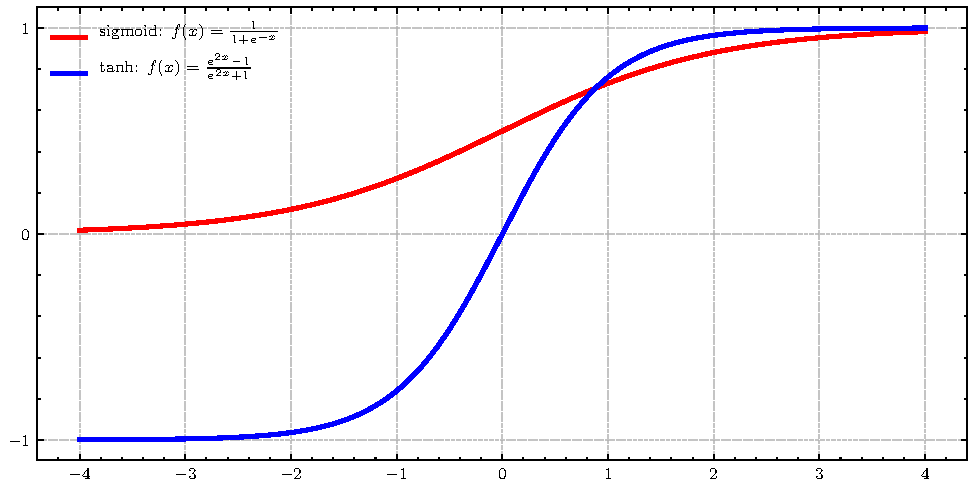
\includegraphics[width=.7\textwidth]{activations.pdf}
  % \medskip
  \caption{Typical activation functions used at the output of convolutional autoencoders.}
  \label{fig:ae_output_fx}
\end{figure}
To accommodate such output functions, most works in both image compression and CSI estimation typically apply \emph{minmax normalization}, where the extrema (i.e., the minimum and the maximum) of the real and imaginary channels are used to scale the entire dataset. For the scalar $H_n(i,j)$, the minmax-scaled version of this element is
\begin{align*}
	H_{n,\text{minmax}}(i,j) &= \frac{H_n(i,j)-H_{\text{min}}}{H_{\text{max}}-H_{\text{min}}} \in [0,1],
\end{align*}
for $n \in [1,\dots,N]$ given a dataset of $N$ samples and $i/j$ indexing the rows/columns of the CSI matrices. The resulting samples are cast to the range $[0,1]$. % Most work in deep learning for CSI estimation focuses on different neural network architectures, training frameworks, or hyperparameter tuning. Such works treat the real and imaginary elements of $\mathbf H$ as separate channels similar to color channels in images.

For image data, minmax normalization results in each image's color channels scaled to the range $[0,1]$. The resulting distribution for each color channel is typically satisfactory for image tasks, as the variance is not much smaller than the range of the normalized data (see Fig.~\ref{fig:imagenet_dist}).

However, for CSI matrices, minmax normalization is applied to the real and imaginary channels of each element. For typical channel models and parameters, the distribution of channel elements tends to have much lower variance than that of image data (see Fig.~\ref{fig:cost_indoor_dist}). This smaller variance can be explained by the difference in the datasets' ranges -- while the channels in image data (e.g., ImageNet) assume integer values between $[0,255]$, the channels in CSI data (e.g., COST2100) assume floating point values smaller than $10^{-3}$.

\begin{figure}[htb]
	\centering
	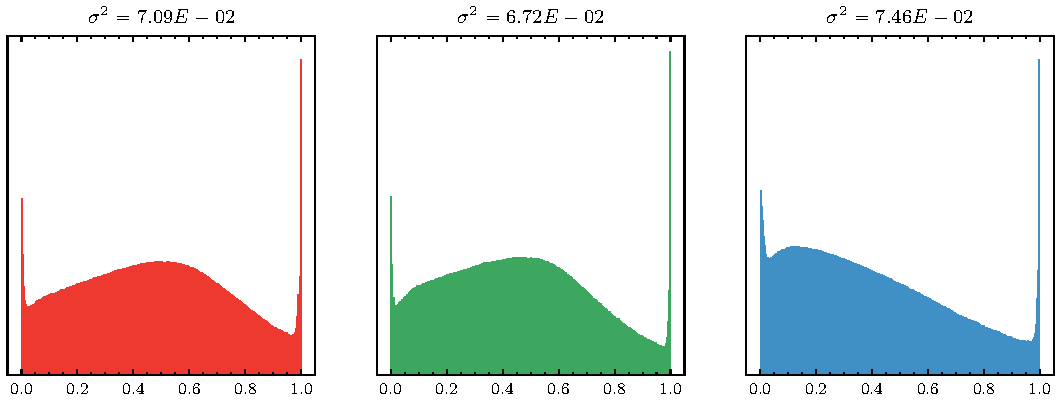
\includegraphics[width=.9\textwidth]{imagenet_rgb_dist.pdf}
	\medskip
	\caption{Distribution and variance of minmax-normalized ImageNet color channels ($N=50000$) images.}
	\label{fig:imagenet_dist}
\end{figure}

\begin{figure}[htb]
	\centering
	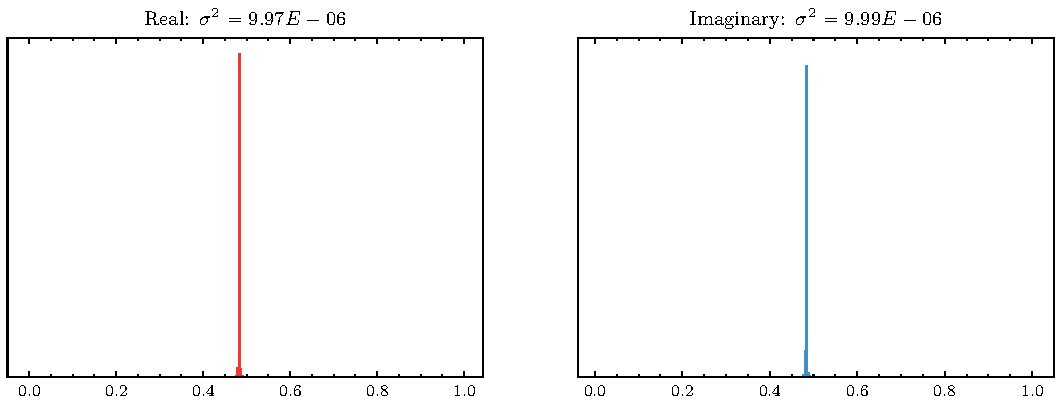
\includegraphics[width=.9\textwidth]{cost2100_indoor_dist.pdf}
	\medskip
	\caption{Distribution and variance of minmax-normalized COST2100 real/imaginary channels ($N=99000$) images.}
	\label{fig:cost_indoor_dist}
\end{figure}

\section{Related Work}

In image processing, several works have investigated normalization techniques such as batch normalization \cite{ref:ioffe2015batch}, instance normalization \cite{ref:huang2017instance}, layer normalization \cite{ref:ba2016layer}, and group normalization \cite{ref:wu2018group}. These normalization techniques scale the outputs of latent layers in neural networks, which helps to solve the problem of covariate shift \cite{ref:ioffe2015batch} where the mean and variance of changes between subsequent layers of the network.

Other works have studied normalization of the network's inputs. A number of works have investigated adaptive normalization techniques for time series estimation tasks \cite{ref:ogasawara2010adaptive, ref:nayak2014impact, ref:shao2015self}. In \cite{ref:passalis2019dain}, the authors proposed a trainable input network which learns to shift, scale, and filter the unnormalized data while training the target network for a time series prediction task.

\section{Spherical Normalization} \label{sect:sph_norm}

Here, we discuss our work in spherical normalization (Section~\ref{sect:sph_norm_method}) and our optimized network architecture, CsiNet-Pro (Section~\ref{sect:csinet_pro}) \cite{ref:liu2020sphnet}.

% \subsection{Spherical Normalization}
\label{sect:sph_norm_method}
Rather than apply minmax normalization, which is adversely impacted by outliers, we propose spherical normalization. Before describing spherical normalization in detail, consider z-score normalization. Given a random variable, $x$, with mean $\mu$ and standard deviation $\sigma$. The z-score normalized version of this random variable is given as
\begin{align}
	z &= \frac{x - \mu}{\sigma^2}. \label{eq:zscore}
\end{align}
Assuming $x$ is normally distributed, the resulting random variable, $z$, is a standard normal distribution such that $z \sim \mathcal N(0,1)$. Inspired by $z$-score normalization, we seek a normalization scheme which adjusts the range of each channel sample. Under spherical normalization, each sample in the dataset is scaled by its power. Denote the $n$-th downlink CSI matrix of the dataset as $\mathbf H_d^n$. The spherically normalized version of the downlink CSI is given as
% TODO: Does this make sense? "For CSI matrices, we could choose to scale each element by it's mean and by the inverse covariance matrix."
\begin{align}
	\mathbf{\check H}_d^n &= \frac{\mathbf H_d^n}{\|\mathbf H_d^n\|}. \label{eq:sph-intro}
\end{align}
Observe that (\ref{eq:sph-intro}) is similar to (\ref{eq:zscore}) without the mean shift in the numerator\footnote{Since the mean of COST2100 data is $\approx 10^{-10}$, we can safely ignore this mean shift in spherical normalization.} and with the power term of each CSI sample rather than the variance of the entire distribution. After applying (\ref{eq:sph-intro}) to each sample, minmax scaling is applied to the entire dataset. The resulting dataset under spherical normalization can exhibit a larger variance than the same dataset under minmax scaling (compare Fig.~\ref{fig:cost_indoor_sph_dist} with Fig.~\ref{fig:cost_indoor_dist}). 
\begin{figure}[htb]
	\centering
	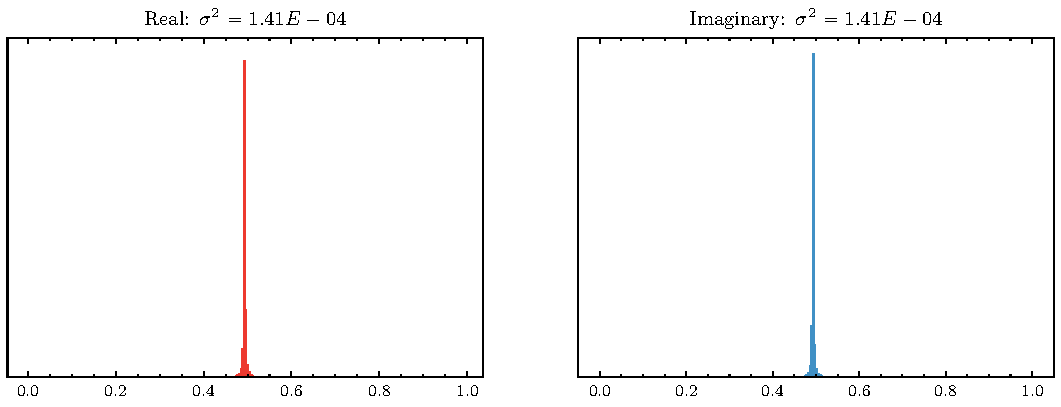
\includegraphics[width=.9\textwidth]{cost2100_indoor_sph_dist.pdf}
	\medskip
	\caption{Distribution and variance of COST2100 real/imaginary channels under spherical normalization ($N=99000$) images.}
	\label{fig:cost_indoor_sph_dist}
\end{figure}

Beyond desirable properties in the input distribution, spherical normalization also results in an objective function which is better matched with the evaluation criterion. Neural networks for CSI estimation are optimized using the mean-squared error loss,
\begin{align} 
	\text{MSE}&=\frac 1N \sum_{k=1}^N\Arrowvert\mathbf H_k - \hat{\mathbf H}_k\Arrowvert^2, \label{eq:mse}
\end{align}
while channel state reconstruction accuracy is measured in terms of normalized mean-squared error,
\begin{align} 
	\text{NMSE}&=\frac 1N \sum_{k=1}^N\frac{\Arrowvert\mathbf H_k - \hat{\mathbf H}_k\Arrowvert^2}{\Arrowvert\mathbf H_k\Arrowvert^2}. \label{eq:nmse}
\end{align}
Observe that when the $\mathbf H_k \; (\hat{\mathbf H}_k)$ in (\ref{eq:mse}) is replaced with $\check{\mathbf H}_k \; (\hat{\check{\mathbf H}}_k)$, we have
\begin{align*} 
	\frac 1N \sum_{k=1}^N\Arrowvert\check{\mathbf H}_k - \hat{\check{\mathbf H}}_k\Arrowvert^2&= \frac 1N \sum_{k=1}^N\left\Arrowvert \frac{\mathbf H_k}{\Arrowvert\mathbf H_k\Arrowvert^2} - \frac{\hat{\mathbf H}_k}{\Arrowvert\mathbf H_k\Arrowvert^2}\right\Arrowvert^2 \\
	&= \frac 1N \sum_{k=1}^N\frac{\Arrowvert\mathbf H_k - \hat{\mathbf H}_k\Arrowvert^2}{\Arrowvert\mathbf H_k\Arrowvert^2},
\end{align*}
which is equivalent to (\ref{eq:nmse}). Thus, a neural network optimized with MSE as the loss function and trained using spherically normalized data is in fact being optimized with respect to NMSE of the original data.

\subsection{CsiNet-Pro}
\label{sect:csinet_pro}

In \cite{ref:liu2020sphnet}, we proposed a network with larger convolutional kernels and no residual connections called CsiNet-Pro. Large kernels (e.g., $(7\times 7)$ in CsiNet-Pro) allow the network to capture features corresponding to larger delay spreads than comparatively small kernels (e.g., $(3\times 3)$ in CsiNet \cite{ref:csinet}). In addition to the compressed feedback of the autoencoder, the encoder must feedback the power of the CSI matrix, $\|H\|$, meaning the number of floating point elements to feed back increases from $r$ to $r+1$.
\begin{figure}[htb]
  \centering
  {
    \fontsize{6pt}{6pt}
    \def\svgwidth{1.0\columnwidth}
    \input{images/csinet-pro.pdf_tex}
  }
  % 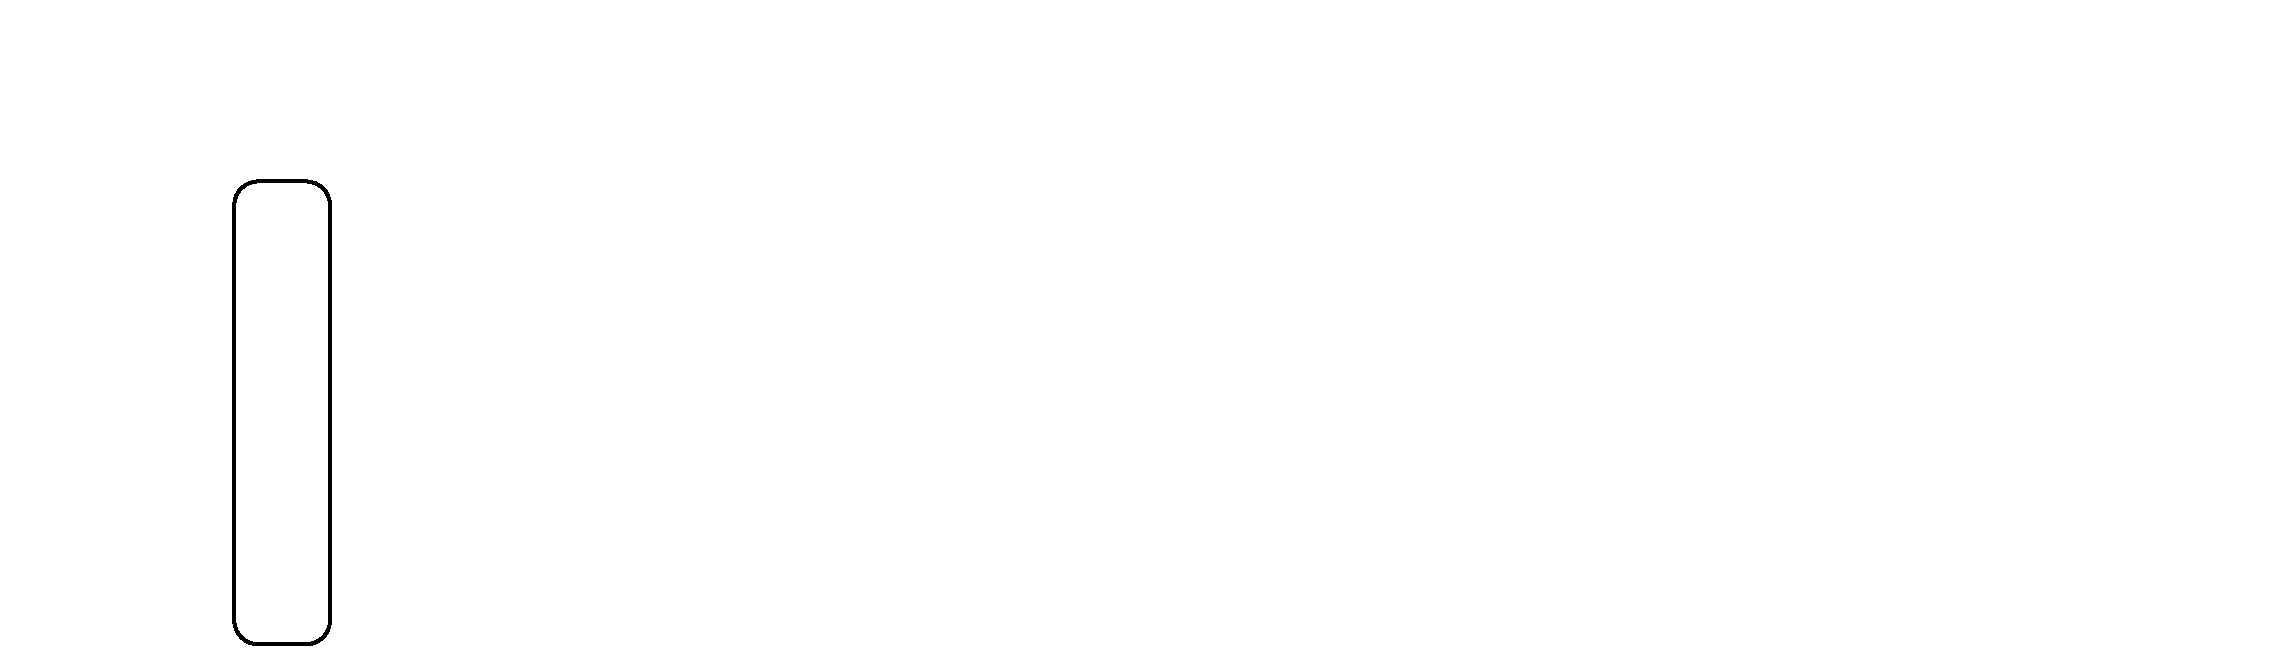
\includegraphics[width=.9\textwidth]{csinet-pro.pdf}
  % \medskip
  \caption{SphNet -- CsiNet-Pro architecture with Spherical Normalization.}
  \label{fig:sphnet-arch}
\end{figure}

\subsection{Results}
Training on spherically normalized data and optimizing with respect to NMSE can yield better accuracy. Fig.~\ref{fig:nmse_slot1} demonstrates this improvement for CsiNet and CsiNet-Pro on the COST2100 dataset. CsiNet and CsiNet-Pro are trained with minmax normalization while CsiNet-Sph and SphNet are trained with spherical normalization. % For both networks, the number of 

\begin{figure}[!hbtp] \centering 
	\begin{subfigure}[t]{.45\textwidth}
		\centering
		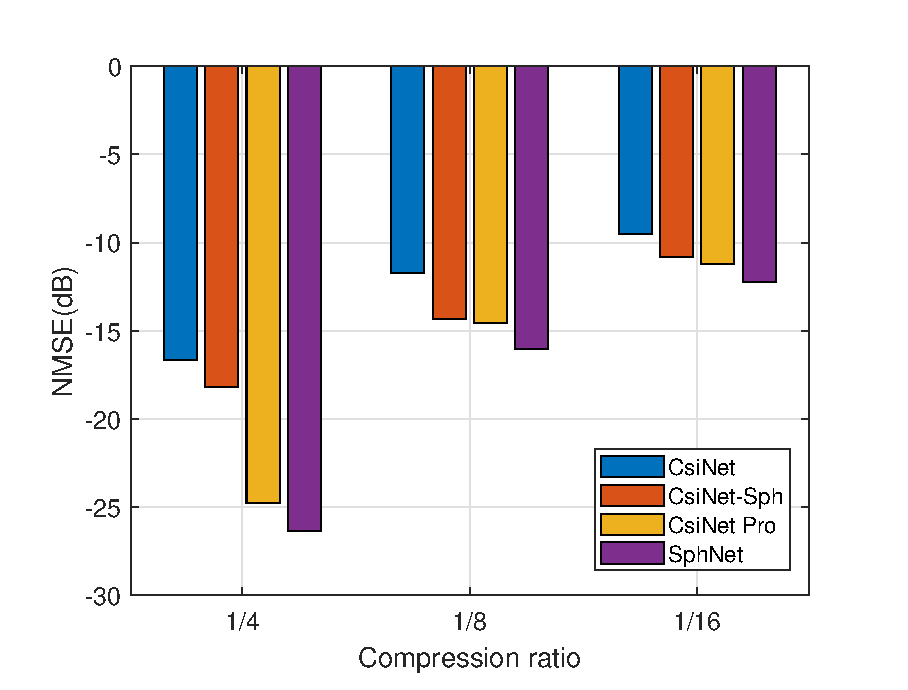
\includegraphics[width=\linewidth]{nmse_slot1_indoor.eps}
		\caption{Indoor}
		\label{fig:slot1_indoor} 
	\end{subfigure}
	\begin{subfigure}[t]{.45\textwidth}
		\centering
		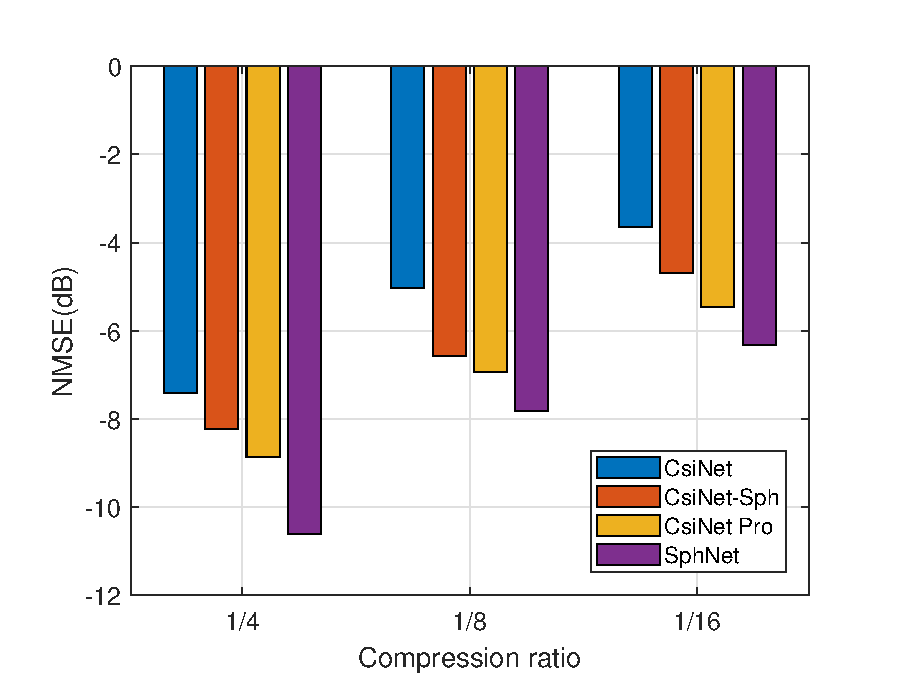
\includegraphics[width=\linewidth]{nmse_slot1_outdoor.eps}
		\caption{Outdoor}
		\label{fig:slot1_outdoor} 
	\end{subfigure}
	\caption{Reconstruction error for CsiNet \cite{ref:csinet} and CsiNet-Pro with and without spherical normalization. SphNet combines CsiNet-Pro with spherical normalization \cite{ref:liu2020sphnet}.}
	\label{fig:nmse_slot1} 
\end{figure}
